%----------------------------------------------------------------------

% Template for TECHNICAL REPORTS at Inst. for Computer Graphics

% and Vision (ICG), Graz University of Technology, Austria:

% style file 'techrep_icg.sty'

%

% author:  Pierre Elbischger

% email:   pierre.elibschger@icg.tu-graz.ac.at

% created: 13.11.2003

% last revision: 25.11.2003

%----------------------------------------------------------------------

% The template contains a number of LaTeX commands of the form :

%

% \command{xyz}

%

% In order to complete this abstract, fill in the blank fields between

% the curly braces or replace already filled in fields with the

% requested information.

%

% e.g. in order to add an abstract title, replace

% \title{}    with   \title{Evidence of Solitons in Tedium Diboride}

%

% The \author and \address commands can take an optional label

% in square brackets of the form :

%

% \command[label]{}

%

% The text of the abstract should be inserted between the two commands

% \begin{abstract} and \end{abstract}.

%

% Please leave all commands in place even if you don't fill them in.

%

%----------------------------------------------------------------------

% Do not alter the following two lines

\documentclass[12pt,a4paper]{article}               % I'm using a double-sided book style

      

\usepackage{techrep_icg}
\usepackage{array}
\usepackage{booktabs}



% package 'graphicx' is automatically included depending on the

%   used compiler (latex, pdflatex), don't include it!!!



\begin{document}

%----------------------------------------------------------------------



%\reportnr{xxx}               % Number of the technical report

\title{Final Report} % Title of technical report

\subtitle{Camera relocalization using regression random forest} % Subtitle of technical report (use small letters only)

\repcity{Graz}            % City where the report was created

\reportnr{1}

\repdate{\today}          % Date of creation

\keywords{Report, Technical report, template, ICG} % keywords that appear below the abstract



%----------------------------------------------------------------------

% List of authors

%

% List each author using a separate \author{} command

% If there is more than one author address, add a label to each author

% of the form \author[label]{name}.  This label should be identical to

% the corresponding label provided with the \address command

% N.B. It is not possible to link an author to more than one address.

%

\author[ICG]{Thomas Pietsch 0930557}
\author[ICG]{Bernhard Rapp 0830250}


%----------------------------------------------------------------------

% List of addresses

%

% If there is more than one address, list each using a separate

% \address command using a label to link it to the respective author

% as described above


\newcommand{\TUGn}{Graz University of Technology}

\address[ICG]{Inst. for Computer Graphics and Vision \\ \TUGn, Austria}



%----------------------------------------------------------------------

% Information about the contact author

% if \contact is not defined (uncommented) or empty, the contact

%  information on the title page is suppressed.



% Name of contact

\contact{Thomas Pietsch}

% Email address of contact - do not use any LaTeX formatting here

\contactemail{thomas.pietsch@student.tugraz.at}



%----------------------------------------------------------------------

% Do not alter the following line



\begin{abstract}



%Replace this text with your abstract.



%----------------------------------------------------------------------

% Do not alter the following two lines

\end{abstract}


\section{Project Proposal}

\subsection{Introduction} % (fold)
\label{sub:intro}
First, a regression forest based on the Piotr Dollar toolbox \cite{piotr} will be implemented. The Matlab code for the Piotr Dollar toolbox is readily available and we will adapt the random classification forest to create a regression forest. Therefore the split function and output has to be modified.

Secondly the implementation itself should be evaluated, to make a statement to the general performance of the implementation.

After that the implementation should be used for camera relocalization. Again the dataset should be evaluated. Here not only the evaluation described below is used, but also own dataset. The aim of this work is to show negative examples and find scenarios where the introduced method \cite{shotton} doesn't work as presented.

\subsubsection{Regression Random Forest}
\label{rrf_intro}
The weak learner \ref{eqn:weaklearner} or split function splits the data into a left and right dataset, by thresholding.

\begin{eqnarray}\label{eqn:weaklearner}
  h(\mathbf{p};\mathbf{\theta}_n) = [ f_{\phi_n}(\mathbf{p}) \geq \tau_n ]
\end{eqnarray}

Such a threshold can be optimized by minimization of the objective function

\begin{eqnarray} \label{eqn:objectiv_function}
  Q(S_n,\theta) = V(S_n) - \sum_{d\in\{L,R\}}{\frac{|S_n^d(\theta)|}{|S_n|}V(S_n^d(\theta))}
\end{eqnarray}

\begin{eqnarray}
  V(S) = \frac{1}{|S|} \sum_{(\mathbf{p},\mathbf{m}) \in S}{||\mathbf{m} - \mathbf{\bar m}||_2^2}
\end{eqnarray}

By computing the mean and variance at each leaf, the probability of the output value is given as well as the output value itself is given simply by the mean value.
Because several trees are included in a forest the output of all trees have to be averaged.

\subsection{Implementation} % (fold)
\label{sub:implementation}
To achieve the defined goal, the Piotr Dollar toolbox \cite{piotr} has to be adopted. To be more precise the Objective function as given in \ref{eqn:objectiv_function} was added. Also variance and mean were added as component of the forest structure, while the mean value can be interpreted as the regression result of each tree.

\subsubsection*{Regression Forest} % (fold)
\label{ssub:regression_forest}


% subsubsection regression_forest (end)

\subsubsection{Evaluation} % (fold)
\label{ssub:camera_relocalization}
First the implementation of a general Random Regression Forest was evaluated. To keep things simple, simple 2D functions were used to calculate an error as well as a visualization.
Some attributes were kept constant:
maxDepth = 50
minChild = 1

While other were changed and performed differently as shown in table %\ref{tab:res_gen}



\begin{tabular}{|c|c|c|c|}
\toprule
Datapoints & \multicolumn{3}{c}{trees} \\ \hline
\midrule
& 50 & 150 & 1500 \\ \hline
1000 & 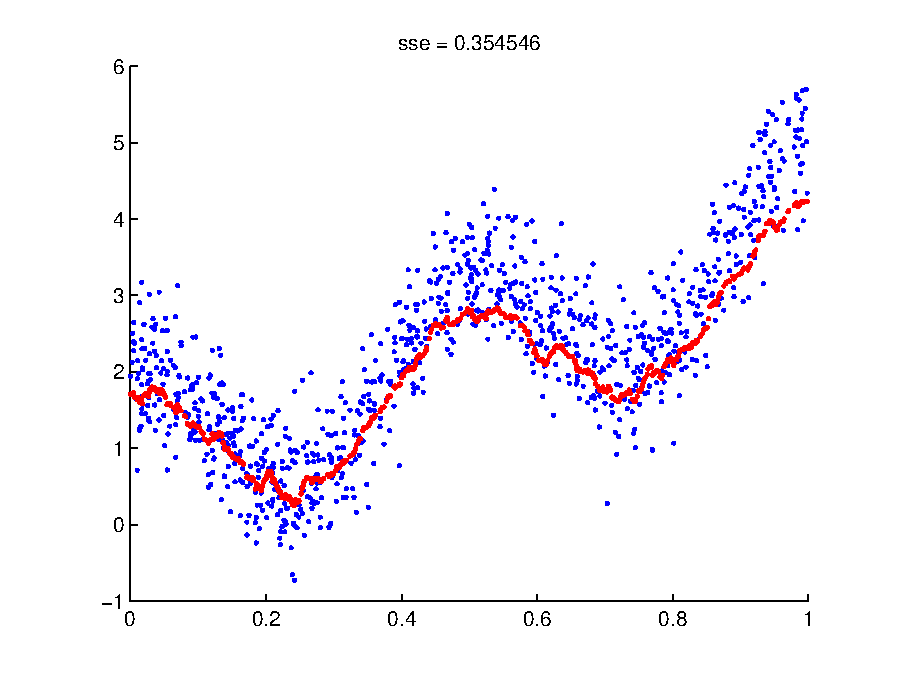
\includegraphics[width=0.25\textwidth]{fig/cos_1k_50} & 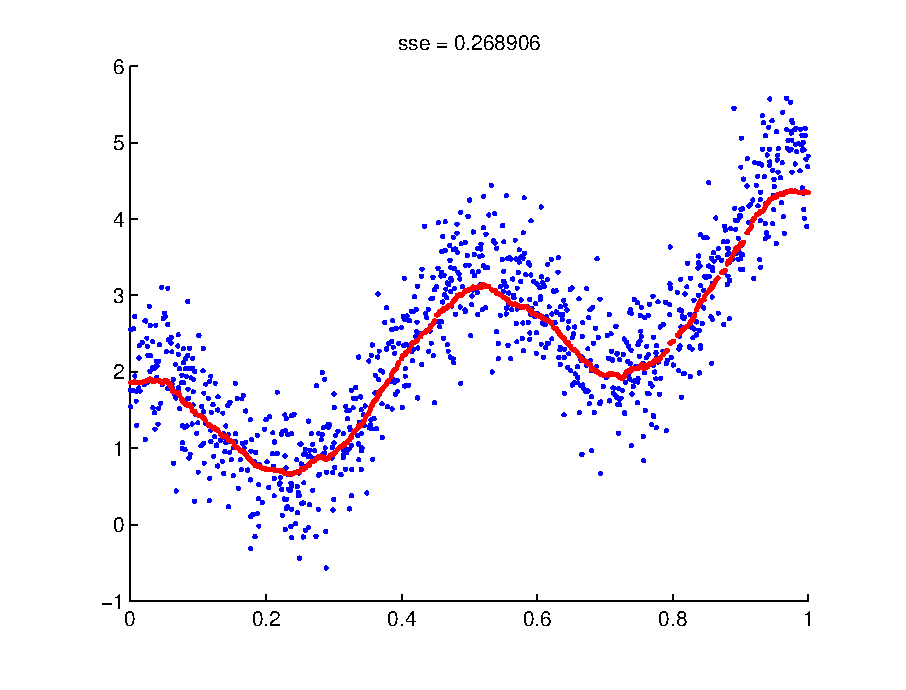
\includegraphics[width=0.25\textwidth]{fig/cos_1k_150} & 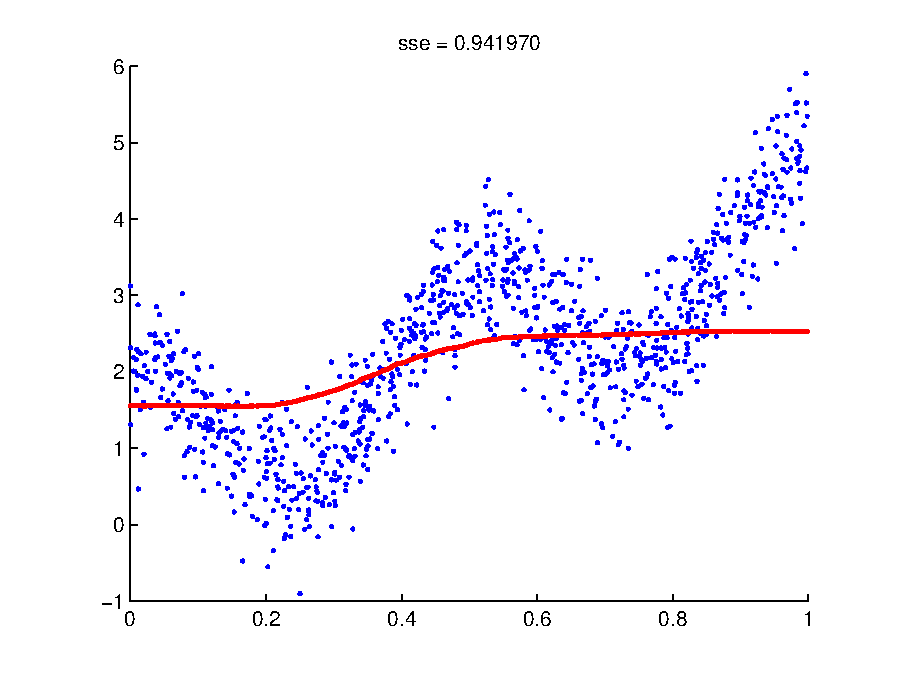
\includegraphics[width=0.25\textwidth]{fig/cos_1k_1500} \\ \hline
10000& 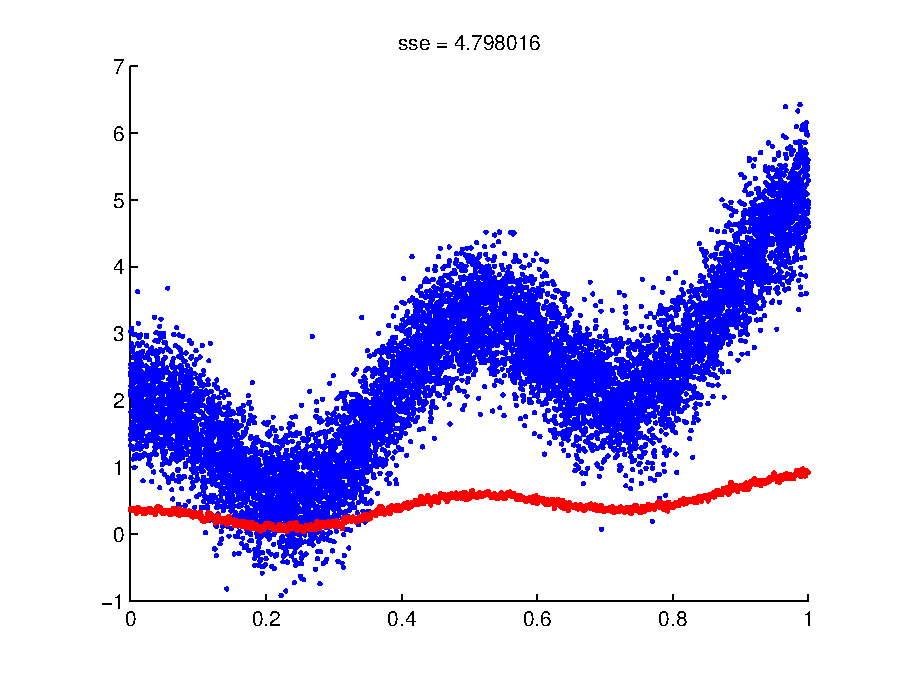
\includegraphics[width=0.25\textwidth]{fig/cos_10k_50} & 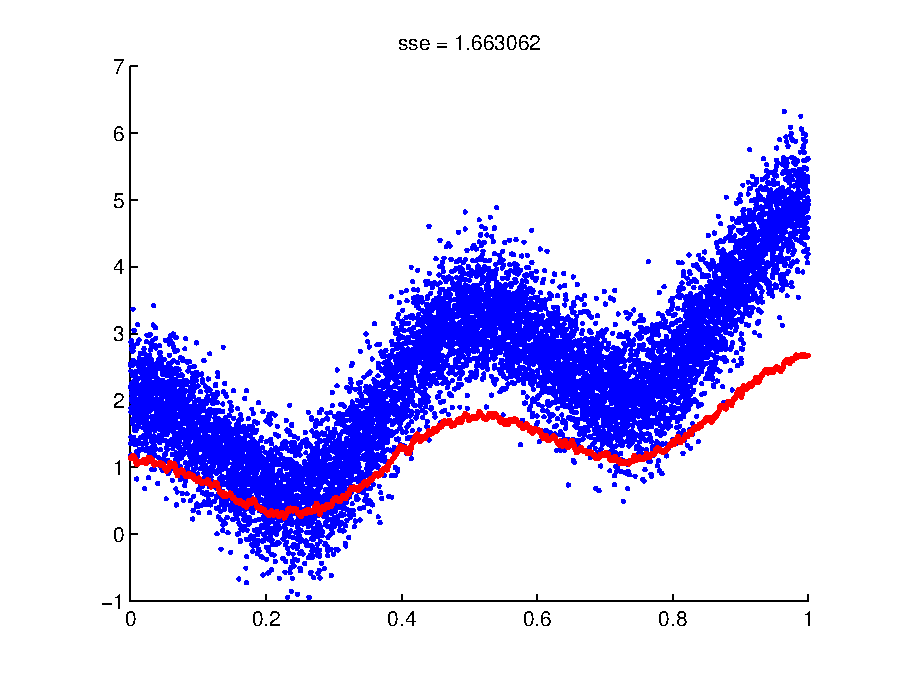
\includegraphics[width=0.25\textwidth]{fig/cos_10k_150} & 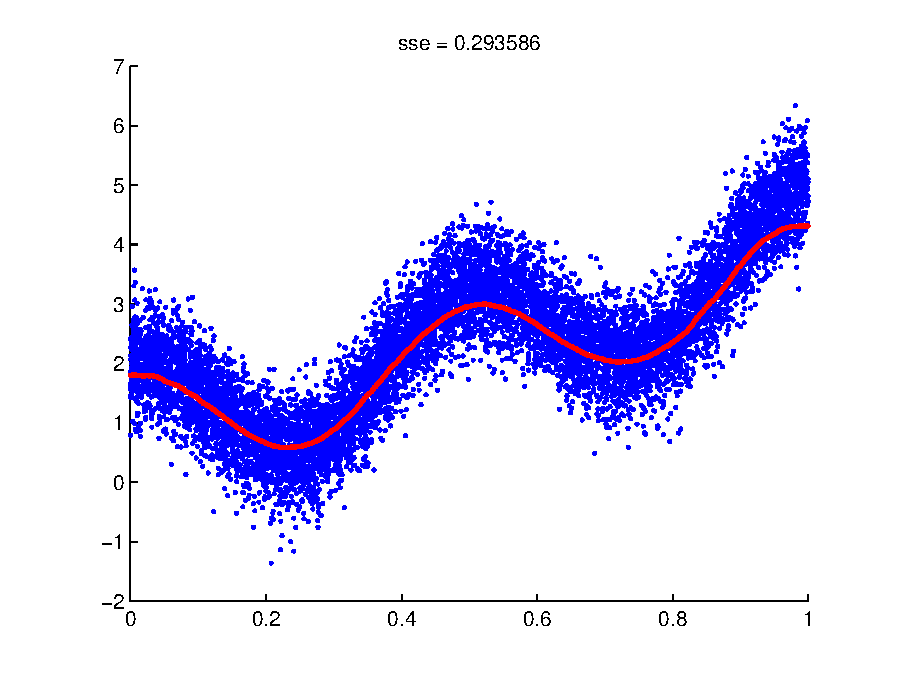
\includegraphics[width=0.25\textwidth]{fig/cos_10k_1500} \\ \hline
\bottomrule
\end{tabular}

%\begin{tabular}{l | c | c}
%\diaghead{\theadfont Diag ColumnmnHead II}%
%{Diag\\Column Head I}{Diag Column\\Head II}&
%datapoints & 50 & 150 & 1500 %& \hline \hline
%\end{tabular}


% subsubsection camera_relocalization (end)

% subsection what_method_will_get_implemented_ (end)




% subsection how_can_the_method_be_evaluated_ (end)


% ============================================================
% Bibliography
% ============================================================
\clearpage
\renewcommand{\leftmark}{}



\bibliographystyle{plain}
%\addcontentsline{toc}{chapter}{Bibliography}
%\bibliographystyle{plain}
\bibliography{./bibtex}

\end{document}

%----------------------------------------------------------------------

